% !TEX root = USEGUIDE.tex

\part{CLASS : General overview}
\chapter{Generalities}
\section{Basic unit\label{sec:cSecond}}
Time in CLASS should be written in second. A special C++  type has been defined for this purpose :  cSecond. This is a  \textbf{long long int}.
Power is always considered as thermal power in watt.
Masses are in metric tons except for molar masses (in gram).
Burnup is in units of GWd/tHM. With tHM stands for metric tons of heavy metal. 
 \section{CLASS working process principle}
image : sh�ma de principe de class
\chapter{Facilities descriptions}
All the facilities in CLASS  are regrouped inside a mother class called CLASSFacility (and inherit of all the properties of the CLASSFacility in a C++ way). Inside the CLASSFacility, 3 different types has been defined, the Reactor, the FabricationPlant (or more generally, all the fuel cycle front-end facilities) and the facilities of the back end of the fuel cycle. 
\section{CLASSFacility\label{sec:CLASSFacility}}
The CLASSFacility should never be used directly in the main CLASS program (the one made to perform the simulation).  The aim of this object is to regroup all the common properties of the nuclear facilities, such as common variables, methods, and builder. 


\section{Reactor\label{sec:reactor}}
\subsection{Generalities}
The aim of this class is to deal with the evolution of the fuel inside a reactor.\\
The evolution of the fuel is \textbf{always} contain in the \hyperref[sec:EvolutionData]{EvolutionData} \textit{fEvolutionDB}.\\
There are 2 way to provide the \hyperref[sec:EvolutionData]{EvolutionData} to the reactor. In the case of fixed fuel\footnote{Always the same input/output isotopic composition.} the user need to provide it, using the appropriated constructor, the set function, or a \hyperref[sec:CLASSFuelPlan]{CLASSFuelPlan}. In the case of recycled fuel or unfixed fuel, the user need to provide a \hyperref[sec:PhysicsModels]{PhysicsModels}, using the appropriated constructor, the set function, and/or a \hyperref[sec:CLASSFuelPlan]{CLASSFuelPlan}.

\subsection{Use}
There are 2 main ways to define a reactor, depending on the type of fuel loaded.

\subsubsection{Fixed Fuel}
Reactor using fixed fuel, which load always the same fresh fuel, and irradiates it to the same burnup (same spent fuel composition), can be declared as follow:
\begin{center}
\begin{minipage}{\textwidth}
\begin{lstlisting}[style=customc]
Reactor *MyReactor = new reactor(aCLASSLogger,		// CLASSLogger
				 myFuel_EvolutionData,	// EvolutionData
				 aBackEnd,		// BackEnd
				 myRe_StartingTime,	// Starting Time
				 myRe_LifeTime,		// Time of Life
				 myRe_Power,		// Power
				 myRe_HeavyMetalMass,	// HM mass
				 myRe_BurnUp,		// BurnUp
				 myRe_LoadFactor);	// LoadFactor
\end{lstlisting}
\end{minipage}
\end{center}
or
\begin{center}
\begin{minipage}{\textwidth}
\begin{lstlisting}[style=customc]
Reactor *MyReactor = new reactor(aCLASSLogger,		// CLASSLogger
				 myFuel_EvolutionData,	// EvolutionData
				 aBackEnd,		// BackEnd
				 myRe_StartingTime,	// Starting Time
				 myRe_LifeTime,		// Time of Life
				 myRe_CycleTime,	// Time of Cycle
				 myRe_HeavyMetalMass,	// HM mass
				 myRe_BurnUp);		// BurnUp
\end{lstlisting}
\end{minipage}
\end{center}
The meaning of each arguments of the two constructor previously defined are summed up in the following table

\begin{table}[H]
\begin{center}
\caption{Arguments of Reactor constructors}
\label{tab:meanKeyWord}
\begin{tabular}{|c|c|c|c|}
\hline
Argument & type & meaning & unit \\
\hline
aCLASSLogger 		&	\hyperref[sec:CLASSLogger]{CLASSLogger}		& Output messages 			& N.A.\\
myFuel\_EvolutionData	&	\hyperref[sec:EvolutionData]{EvolutionData}	& Fuel evolution description		& N.A. \\
aBackEnd 		&	\hyperref[sec:CLASSBackEnd]{CLASSBackEnd}	& Facility getting the spent fuel 	& N.A. \\
myRe\_StartingTime 	&	\hyperref[sec:cSecond]{cSecond}			& Creation time 			& second\\
myRe\_LifeTime 		&	\hyperref[sec:cSecond]{cSecond}			& Operation time 			& second\\
myRe\_Power 		&	double						& Thermal power 			& Watt\\
myRe\_HeavyMetalMass 	&	double						& Heavy metal mass 			& tons\\
myRe\_BurnUp 		&	double						& Burn up at EOC 			& GWd/tHM\\
myRe\_LoadFactor 	&	double						& Fraction of nominal power 		& .\\
myRe\_CycleTime 	&	\hyperref[sec:cSecond]{cSecond}			& the cycle time 			& second\\
\hline
\end{tabular}
\end{center}
\end{table}


\subsubsection{Reprocessed Fuel}
In this case, the fuel is provided by an external facility, so called, the \hyperref[sec:FabricationPlant]{FabricationPlant}. The way to build the reprocessed fresh fuel and to handle the fuel depletion calculation is done by the \hyperref[sec:PhysicsModels]{PhysicsModels}.
The main ways to defined a Reactor (with reprocessed fuel) are shown in the next two examples :

\begin{center}
\begin{minipage}{\textwidth}
\begin{lstlisting}[style=customc]
Reactor *MyReactor = new Reactor(aCLASSLogger,		// CLASSLogger
				 myFuel_PhysicsModels,	// PhysicsModels
				 aFabricationPlant,	// FabricationPlant
				 aBackEnd,		// BackEnd
				 myRe_StartingTime,	// Starting Time
				 myRe_LifeTime,		// Time of Life
				 myRe_Power,		// Power
				 myRe_HeavyMetalMass,	// HM mass
				 myRe_BurnUp,		// BurnUp
				 myRe_LoadFactor);	// LoadFactor
\end{lstlisting}
\end{minipage}
\end{center}
or
\begin{center}
\begin{minipage}{\textwidth}
\begin{lstlisting}[style=customc]
Reactor *MyReactor = new Reactor(aCLASSLogger,		// CLASSLogger
				 myFuel_PhysicsModels,	// PhysicsModels
				 aFabricationPlant,	// FabricationPlant
				 aBackEnd,		// BackEnd
				 myRe_StartingTime,	// Starting Time
				 myRe_LifeTime,		// Time of Life
				 myRe_CycleTime,	// Time of Cycle
				 myRe_HeavyMetalMass,	// HM mass
				 myRe_BurnUp);		// BurnUp
\end{lstlisting}
\end{minipage}
\end{center}
The meaning of each argument of the two constructors previously defined are summed up in the following table

\begin{table}[H]
\begin{center}
\caption{Arguments of Reactor constructors}
\label{tab:meanKeyWord}
\begin{tabular}{|c|c|c|c|}
\hline
Argument & type & meaning & unit \\
\hline
aCLASSLogger 		& \hyperref[sec:CLASSLogger]{CLASSLogger}		& Output messages 			& N.A.\\
myFuel\_PhysicsModels	& \hyperref[sec:PhysicsModels]{PhysicsModels}		& Fuel construction/evolution		& N.A. \\
aFabricationPlant 	& \hyperref[sec:FabricationPlant]{FabricationPlant}	& Facility building the fuel 		& N.A. \\
aBackEnd 		& \hyperref[sec:CLASSBackEnd]{CLASSBackEnd}		& Facility getting the spent fuel 	& N.A. \\
myRe\_StartingTime 	& \hyperref[sec:cSecond]{cSecond}			& Creation time 			& second\\
myRe\_LifeTime 		& \hyperref[sec:cSecond]{cSecond}			& Operation time 			& second\\
myRe\_Power 		& double						& Thermal power 			& Watt\\
myRe\_HeavyMetalMass 	& double						& Heavy metal mass 			& tons\\
myRe\_BurnUp 		& double						& Burn up at EOC 			& GWd/tHM\\
myRe\_LoadFactor 	& double						& Fraction of nominal power 		& .\\
myRe\_CycleTime 	& \hyperref[sec:cSecond]{cSecond}			& the cycle time 			& second\\
\hline
\end{tabular}
\end{center}
\end{table}

\subsection{CLASSFuelPlan}
A reactor may changes of fuel type during its lifetime. To handle this, the user can destroy the reactor and build a new one with an other kind of fuel. In order to make the process more flexible, the CLASSFuelPlan has been added to the CLASS package. The following example explains how to make a reactor to change its fuel type and burn-up.
\begin{center}
\begin{minipage}{\textwidth}
\begin{lstlisting}[style=customc]
Reactor* MyReactor = new Reactor(gCLASS->GetLog(),        //Log
                                        EvolutionData0,            // DB
                                        Stock,                 // BackEnd
                                        StartingTime,      // Starting time
                                        LifeTime,            // Time of life
                                        Power_CP0,       // Power
                                        HMMass,    // HM mass
                                        BU0,            // BurnUp
                                        0.8);  //Load factor
                                        
MyReactor->GetFuelPlan()->AddFuel( ChangingFuelTime0, EvolutionData1, BU1);
MyReactor->GetFuelPlan()->AddFuel( ChangingFuelTime1, PhyMod, BU2);
\end{lstlisting}
\end{minipage}
\end{center}
At \emph{ChangingFuelTime0} the reactor changes its fuel from \emph{EvolutionData0} to \emph{EvolutionData1} and its Burn-up from \emph{BU0} to \emph{BU1}. At \emph{ChangingFuelTime1}, the reactor uses reprocessed fuel using the \hyperref[sec:PhysicsModels]{PhysicsModels}  \emph{PhyMod}.

\section{CLASSBackEnd\label{sec:CLASSBackEnd}}
The CLASSBackEnd class is a mother class which aims to regroup all common properties of the facilities of the back end of the fuel cycle.\\
A CLASSBackEnd does not control its upstream. Its incoming material flux is pushed by its upstream facility (a Reactor, or an other CLASSBackEnd). It only controls its downstream flux.\\
\textbf{This object is not supposed to be used explicitly in a CLASS input.}
\subsection{Storage}\label{sec:Storage}
Storage is a CLASSBackEnd without associated downstream factory. All the incoming material are stored individually in different \hyperref[sec:IsotopicVector]{IsotopicVector} (see figure~\ref{fig:StorageIV}). During the storage, the depletion by decay is taken into account. The storage has to be defined as follow :
\begin{center}
\begin{minipage}{\textwidth}
\begin{lstlisting}[style=customc]
Storage *Stock = new Storage(aCLASSLogger);
\end{lstlisting}
\end{minipage}
\end{center}
 
\begin{figure}[H]
\centering
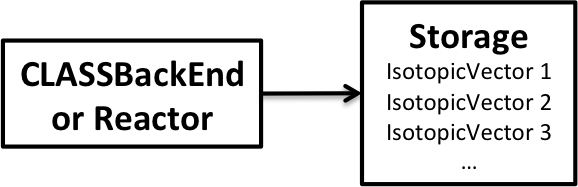
\includegraphics[width=0.4\textwidth]{Storage_IV.png} 
\caption{ Storage \label{fig:StorageIV} }
\end{figure} 
 
\subsection{Pool\label{sec:pool}}
Pool is a CLASSBackEnd with an associated downstream factory. All incoming material will be pushed in the downstream factory after a certain cooling time.  All the incoming material are stored individually in different \hyperref[sec:IsotopicVector]{IsotopicVector} (the same way as the \hyperref[sec:Storage]{Storage}) . During the cooling process, the depletion by decay is taken into account. The Pool has to be defined as follow :
\begin{center}
\begin{minipage}{\textwidth}
\begin{lstlisting}
Pool *MyPool = new Pool(aCLASSLogger, aCLASSBackEnd, 5*365.25*24.*3600);
\end{lstlisting}
\end{minipage}
\end{center}
In the previous example, a 5 years cooling time has been used.
If no downstream facility is set, all the material will be sent, after the cooling time, to the WASTE of the Scenario. To do so :
\begin{center}
\begin{minipage}{\textwidth}
\begin{lstlisting}[style=customc]
Pool *MyPool = new Pool(aCLASSLogger, 5*365.25*24.*3600);
\end{lstlisting}
\end{minipage}
\end{center}

\subsection{SeparationPlant\label{sec:SeparationPlant}}
The role of the SeparationPlant is to separate an incoming \hyperref[sec:IsotopicVector]{IsotopicVector} from a facility into an arbitrary number of outgoing \hyperref[sec:CLASSBackEnd]{CLASSBackEnd}.\\
To define a SeparationPlant proceed as follow :
\begin{center}
\begin{minipage}{\textwidth}
\begin{lstlisting}[style=customc]
SeparationPlant* MySeparationPlant = new SeparationPlant(aCLASSLogger);
\end{lstlisting}
\end{minipage}
\end{center}

The separation process is instantaneous and it uses isotopic separation efficiencies. Efficiencies must be given as an \hyperref[sec:IsotopicVector]{IsotopicVector} containing the separation efficiency for each nucleus. Note that it is possible to separate the incoming \hyperref[sec:IsotopicVector]{IsotopicVector} in many, the users must provide as many isotopic separation efficiency as outgoing \hyperref[sec:CLASSBackEnd]{CLASSBackEnd}.\\
In addition of an outgoing CLASSBackEnd and an associated isotopic separation efficiency, the user must provide a date for the separation to be effective. To do so :
\begin{center}
\begin{minipage}{\textwidth}
\begin{lstlisting}[style=customc]
IsotopicVector IV_MA; //Define Minor Actinides (MA) separation efficiencies
IV_MA.Add(93, 237, 0, 1.);
IV_MA.Add(95, 242, 1, 1.);
IV_MA.Add(96, 245, 0, 1.);
//...
MySeparationPlant->SetBackEndDestination(aCLASSBackEnd1 //destination of MA
					IV_MA, //Efficiencies
					2000*365.25*24.3600);//Time when the separation begin

IsotopicVector IV_Pu; //Defined Plutonium separation efficiencies
IV_Pu.Add(94, 238, 0, 0.8);
IV_Pu.Add(94, 239, 0, 0.8);
//...
MySeparationPlant->SetBackEndDestination(aCLASSBackEnd2, 
					IV_Pu, 
					2005*365.25*24.3600);
					
IsotopicVector IV_U;
IV_U += 0.5*ZAI(92, 235, 0);
IV_U += 0.5*ZAI(92, 238, 0);
//...
MySeparationPlant->SetBackEndDestination(aCLASSBackEnd3, 
					IV_U, 
					2015*365.25*24.3600);
\end{lstlisting}
\end{minipage}
\end{center}
In the present example defined above, the separation of Minor Actinides start in 2000, this separated material is sent to the CLASSBackEnd \textit{aCLASSBackEnd1} (the rest goes to the WASTE). The separation of the plutonium start in 2005 (the separated Pu is sent to \textit{aCLASSBackEnd2}) and the separation of uranium take place in 2010.\\
Note that between 2005 and 2010, both MA and Pu are separated and sent respectively to \textit{aCLASSBackEnd1} and \textit{aCLASSBackEnd2}, all the remaining isotopes are sent to the WASTE. After 2010, MA, Pu and U are separated and sent to their respective CLASSBackEnd facilities, the rest is still sent to WASTE.\\
Furthermore, the separation of Actinides Minor has an efficiency of 100\%, Pu of 80\% and U of 50\%.
Please refer to \$CLASS\_PATH/example/Separation.cxx for a simple CLASS input using the SeparationPlant.


\section{Fabrication Plant\label{sec:FabricationPlant}}
The FabricationPlant is the facility which takes care of the fuel fabrication. The "action" in FabricationPlant appends before the beginning of cycle of a reactor: One fabrication time (Fabrication duration) before the BOC,  the building process of the fuel start.\\
First, the FabricationPlant sorts the different \hyperref[sec:IsotopicVector]{IsotopicVector}s in the different inputs  \hyperref[sec:Storage]{Storage} according to the user priorities. Then, it asks the \hyperref[sec:EquivalenceModel]{EquivalenceModel} of the \hyperref[sec:PhysicsModels]{PhysicsModels} associated to the reactor how to build a fuel with the correct properties using the available \hyperref[sec:IsotopicVector]{IsotopicVector}s contained in the \hyperref[sec:Storage]{Storage}. The \hyperref[sec:EquivalenceModel]{EquivalenceModel} provide a list of fraction to take in each \hyperref[sec:IsotopicVector]{IsotopicVector}s in the Storage . According to this fraction list, the FabricationPlant takes the fraction in each \hyperref[sec:IsotopicVector]{IsotopicVector} and build the reprocessed fuel.
Once the reprocessed fuel is made, it asks the PhyscisModel to calculate its depletion and store the result in an \hyperref[sec:EvolutionData]{EvolutionData}.  The reactor takes this  \hyperref[sec:EvolutionData]{EvolutionData} from the FabricationPlant at its begining of cycle.\\
Between the fuel fabrication and the loading of the fuel in the reactor, the depletion of the fresh fuel by decay is taken into account.\\
Note that, the FabricationPlant provide to the \hyperref[sec:EquivalenceModel]{EquivalenceModel} a list of stock which has virtually decayed for  the fabrication time.

To setup a FabricationPlant do as follow :
\begin{center}
\begin{minipage}{\textwidth}
\begin{lstlisting}[style=customc]
FabricationPlant *MyFabricationPlant = new FabricationPlant(gCLASS->GetLog(), 1*year);
MyFabricationPlant->SetFiFo();
\end{lstlisting}
\end{minipage}
\end{center}

In the previous example, the SetFifo() method set the first in first out priority for the stock usage. It means that the older \hyperref[sec:IsotopicVector]{IsotopicVector} of the Storage is taken in priority by the FabricationPlant. If the younger \hyperref[sec:IsotopicVector]{IsotopicVector} is wanted to be taken in priority : one should use SetFiFo(false).

The Storage used to extract the fissile part of the fuel is set using :
\begin{center}
\begin{minipage}{\textwidth}
\begin{lstlisting}[style=customc]
MyFabricationPlant->AddFissileStorage(Stock);
\end{lstlisting}
\end{minipage}
\end{center}
And if necessary it is possible to define a  \hyperref[sec:Storage]{Storage} where  fertile isotopes will be extracted, using :
\begin{center}
\begin{minipage}{\textwidth}
\begin{lstlisting}[style=customc]
MyFabricationPlant->AddFertileStorage(Stock);
\end{lstlisting}
\end{minipage}
\end{center}
If no fertile Storage are defined, the fertile part is taken from outside of the Scenario.
By default the unused part of the stock is sent to WASTE. But it is possible to set a storage where the unused part of the stock will be stored, using :
\begin{center}
\begin{minipage}{\textwidth}
\begin{lstlisting}[style=customc]
MyFabricationPlant->SetReUsableStorage(Stock);
\end{lstlisting}
\end{minipage}
\end{center}

Please refer to \$CLASS\_PATH/example/CloseCycle.cxx for a simple CLASS input using the FabricationPlant
.
\section{Pathway between Facilities}
As explain previously, there are 3 different facility family, the FabricationPlant, the Reactor, and the CLASSBackEnd. All the facilities of type CLASSBackEnd can't get material from other facilities by itself. It is always an other facility which sends material in the CLASSBackEnd. On another hand, some CLASSBackEnd facilities can send material inside other facilities: the SeparationPlant and the Pool. The Storage can only store materials.\\
The reactor takes its fuel from a FabricationPlant and sends the irradiated fuel in a CLASSBackEnd.\\
The FabricationPlant takes its materials from a storage and stored the reprocessed fuel until the beginning of cycle of the Reactor.
In the following, 4 examples of pathways between facilities are listed. These examples are here to illustrate the possible pathways. These examples are not exhaustive. Furthermore, almost any composition between these examples could be made. 


\subsection{Reactor with fixed fuel and a Storage}
Please refer to the CLASS input \$CLASS\_PATH/example/SimpleReactor.cxx
\begin{figure}[h!]
\centering
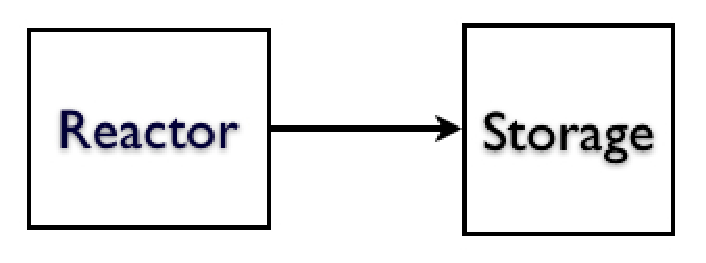
\includegraphics[width=0.4\textwidth]{R-S} 
\caption{Shematic Pathway\label{fig:R-S} }
\end{figure}

\begin{center}
\begin{minipage}{\textwidth}
\begin{lstlisting}[style=customc]
CLASSLogger *Logger = new CLASSLogger("CLASS_OUTPUT.log",1,2);  
EvolutionData* myFuel_EvolutionData = new EvolutionData(Logger, "/PATH/EvolData.dat");

Storage* MyStorage = new Storage(Logger);

Reactor *MyReactor = new Reactor(Logger, myFuel_EvolutionData, MyStorage, 0, 40*365.25*24.3600, 900E6, 100, 45, 1);	
\end{lstlisting}
\end{minipage}
\end{center}

\subsection{Reactor with fixed fuel, a Pool and a Storage}
Please refer to the CLASS input \$CLASS\_PATH/example/SimpleReactor2.cxx
\begin{figure}[h!]
\centering
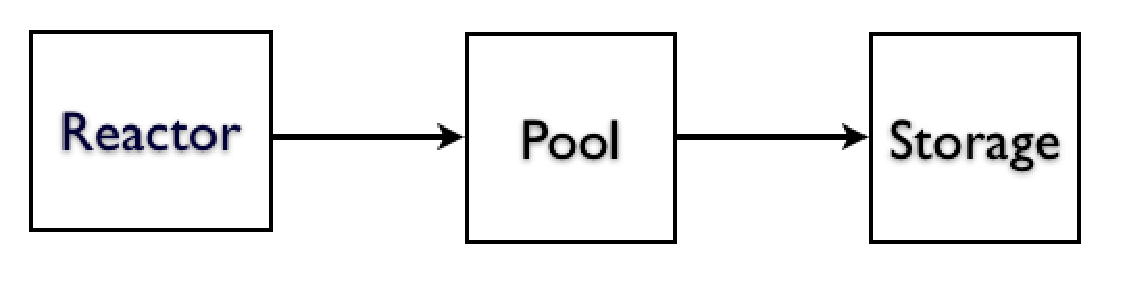
\includegraphics[width=0.6\textwidth]{R-P-S} 
\caption{Shematic Pathway\label{fig:R-P-S} }
\end{figure}

\begin{center}
\begin{minipage}{\textwidth}
\begin{lstlisting}[style=customc]
CLASSLogger *Logger = new CLASSLogger("CLASS_OUTPUT.log",1,2);  
EvolutionData* myFuel_EvolutionData = new EvolutionData(Logger, "/PATH/EvolData.dat");

Storage* MyStorage = new Storage(Logger);
Pool* MyPool = new Pool(Logger, MyStorage, 5*365.25*24*3600);

Reactor *MyReactor = new Reactor(Logger, myFuel_EvolutionData, MyPool, 0, 40*365.25*24.3600, 900E6, 100, 45, 1);	
\end{lstlisting}
\end{minipage}
\end{center}
\pagebreak

\subsection{Reactor with fixed fuel, two SeprationPlant, a Pool and four Storage}
Please refer to the CLASS input \$CLASS\_PATH/example/Separation.cxx
\begin{center}
\begin{minipage}{\textwidth}
\begin{lstlisting}[style=customc]
CLASSLogger *Logger = new CLASSLogger("CLASS_OUTPUT.log",1,2);  
EvolutionData* myFuel_EvolutionData = new EvolutionData(Logger, "/PATH/EvolData.dat");

Storage* MyStorage1 = new Storage(Logger);
Storage* MyStorage2 = new Storage(Logger);
Storage* MyStorage3 = new Storage(Logger);
Storage* MyStorage4 = new Storage(Logger);

Pool* MyPool1 = new Pool(Logger, MyStorage1, 5*365.25*24*3600);

// SeparationPlant separate U5 from U8 which goes in Storage 3 and 4.
SeparationPlant* MySeparation1 = new SeparationPlant(Logger);
IsotopicVector IV_U8;
IV_U8.Add(92, 238, 0, 1);
MySeparationPlant1->SetBackEndDestination(MyStorage3, IV_U8, 0);
					
IsotopicVector IV_U5;
IV_U5 += 1*ZAI(92, 235, 0);
MySeparationPlant1->SetBackEndDestination(MyStorage4, IV_U5, 0);
					

// SeparationPlant separate Am Pu and U which goes respectively in myPool1, myStorage2 and mySeparationPlan1.
SeparationPlant* MySeparation2 = new SeparationPlant(Logger);
IsotopicVector IV_MA;
IV_MA.Add(95, 242, 1, 1.);
MySeparationPlant2->SetBackEndDestination(MyPool1, IV_MA, 0);

IsotopicVector IV_Pu;
IV_Pu.Add(94, 239, 0, 0.8);
MySeparationPlant2->SetBackEndDestination(MyStorage2, IV_Pu, 0);
					
IsotopicVector IV_U;
IV_U.Add(92, 238, 0, 0.5);
IV_U.Add(92, 235, 0, 0.5);
MySeparationPlant2->SetBackEndDestination(MySeparationPlant1, IV_U, 0);

Reactor *MyReactor = new Reactor(Logger, myFuel_EvolutionData, MySeparation2, 0, 40*365.25*24.3600, 900E6, 100, 45, 1);	

\end{lstlisting}
\end{minipage}
\end{center}

\begin{figure}[h!]
\centering
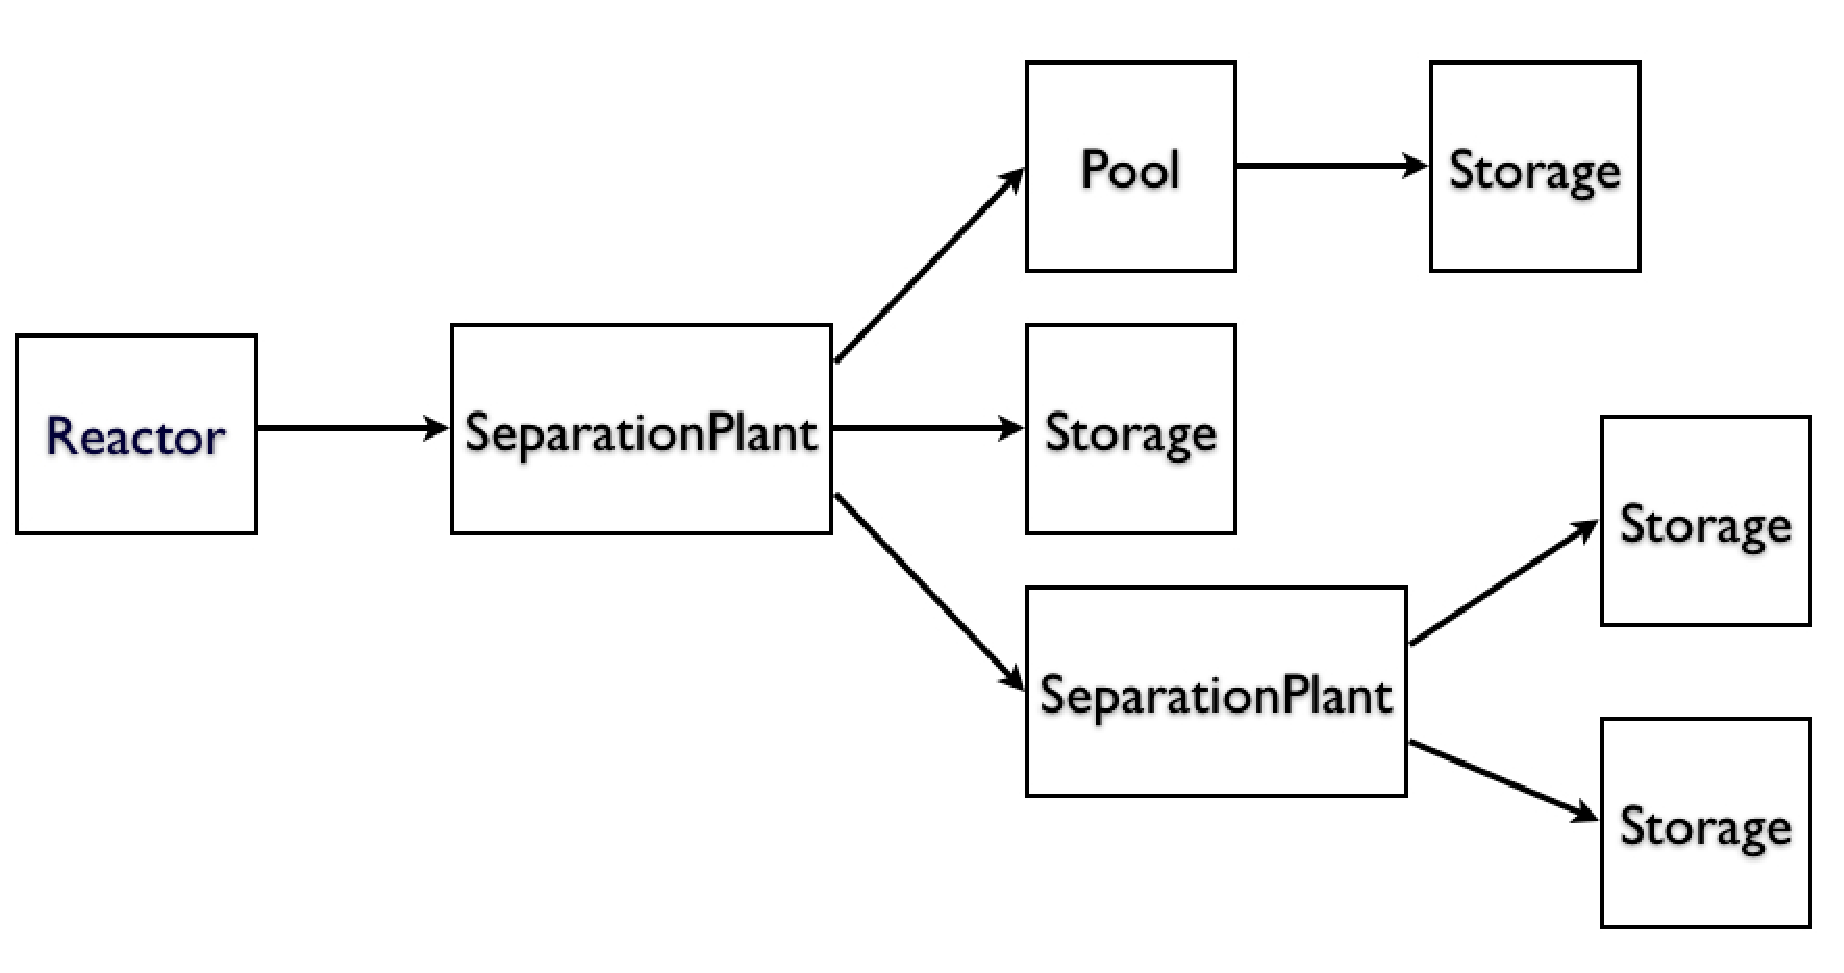
\includegraphics[width=1\textwidth]{R-SP-P_S-S-SP_S_S} 
\caption{Shematic Pathway\label{fig:R-SP-P_S-S-SP_S_S} }
\end{figure}

\pagebreak
\subsection{Reactor, a FabricationPlant, a Pool and a Storage}
Please refer to the CLASS input \$CLASS\_PATH/example/CloseCycle.cxx
\begin{center}
\begin{minipage}{\textwidth}
\begin{lstlisting}[style=customc]
CLASSLogger *Logger = new CLASSLogger("CLASS_OU TPUT.log",1,2);  

IM_RK4 *IMRK4 = new IM_RK4(Logger);
EQM_LIN_PWR_MOX* EQMLINPWRMOX = new EQM_LIN_PWR_MOX(Logger, "/PATH/EQ_Lin.dat");
EQM_QUAD_PWR_MOX* EQMQUADPWRMOX = new EQM_QUAD_PWR_MOX(Logger, "/PATH/DBParam.dat");
PhysicsModels* myFuel_PhysicsModel = new PhysicsModels(XSMOX, EQMQUADPWRMOX, IMRK4);

Storage* MyStorage = new Storage(Logger);
Pool* MyPool = new Pool(Logger, MyStorage, 5*365.25*24*3600);

FabricationPlant* myFabrication = new FabricationPlant(Logger, MyStorage, 2*365.25*24*3600);

Reactor *MyReactor = new Reactor(Logger, myFuel_PhysicsModel, myFabrication, MyPool, 0, 40*365.25*24.3600, 900E6, 100, 45, 1);	
\end{lstlisting}
\end{minipage}
\end{center}
\begin{figure}[h!]
\centering
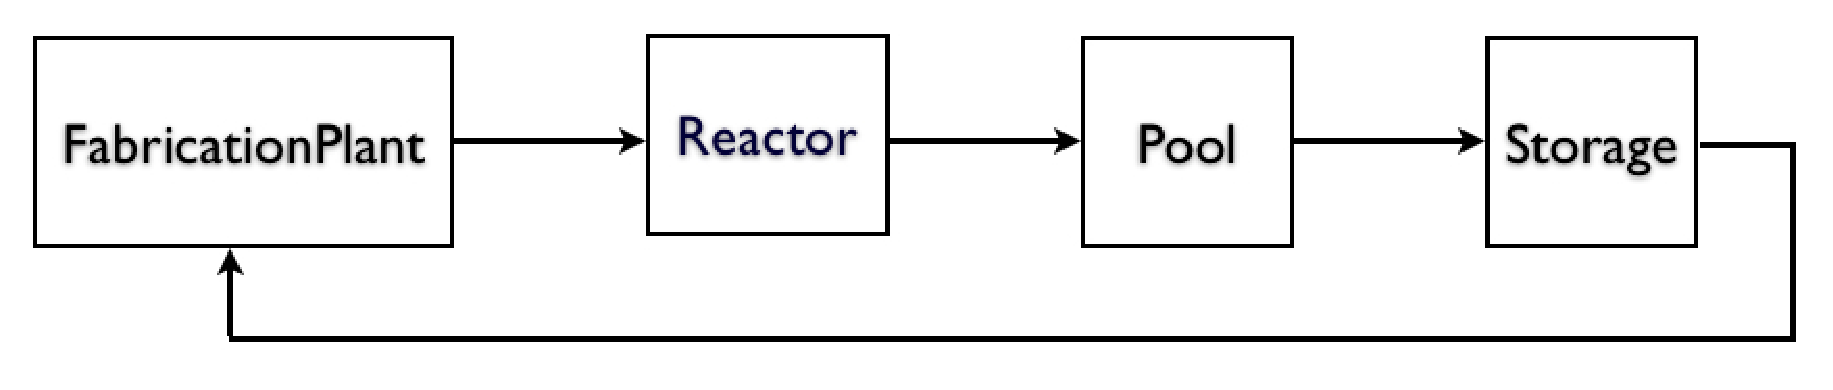
\includegraphics[width=0.9\textwidth]{FP_R_P_S} 
\caption{Shematic Pathway\label{fig:FP_R_P_S} }
\end{figure}

\chapter{Other objects}
\section{ZAI\label{sec:ZAI}}
The ZAi object represents a nucleus, from its charge number, mass number and isomeric state.\\
The object save  the charge number Z, the mass number A and the isomeric state I of a nucleus : I=0 for ground state , I=1 for the first isomeric state ...\\
To declare a ZAI object proceed as follow :
\begin{center}
\begin{minipage}{\textwidth}
\begin{lstlisting}[style=customc]
ZAI U238 = ZAI(92, 238, 0);
\end{lstlisting}
\end{minipage}
\end{center}
This class includes the mains logical comparators (\emph{e.g} ==, >, !=). Fill free to read the \href{https://forge.in2p3.fr/projects/classforge/embedded/doxygen/inherits.html}{ doxygen} for more details on the methods associated to this class. (\emph{e.g} A(), Z(), I(), N()...) .
%\vspace{4cm}

\section{IsotopicVector\label{sec:IsotopicVector}}
\subsection{Generality}
The IsotopicVector object is a collection of ZAI. For each ZAI a quantity of nuclei is associated (IsotopicVector is a c++ map of ZAI and double, which corresponds to a sorted array of ZAI and its quantity).\\
Two main operations have been defined in the IsotopicVector class. 
The following illustrates the possible operations allowed for IsotopicVectors :
\paragraph{Definiton \& Addition of nuclei}
\begin{center}
\begin{minipage}{\textwidth}
\begin{lstlisting}[style=customc]
IsotopicVector IV_1;
IsotopicVector IV_2;

IV_1 += 23 * ZAI(92, 238, 0); // Add 23 nucleus of uranium 238 to ZAI_1
IV_1.Add(92, 235, 0, 52);     // Add 52 nucleus of uranium 235 to ZAI_1
\end{lstlisting}
\end{minipage}
\end{center}
\paragraph{Multiplication}
\begin{center}
\begin{minipage}{\textwidth}
\begin{lstlisting}[style=customc]
IV_1 *= 100; // Multiply all the nuclei quantities by 100 -> resulting : 2300 uranium 238 and 5200 uranium 235

IV_2 = IV_1 * 10; // IV_2 will be equal to 10 IV_1 
\end{lstlisting}
\end{minipage}
\end{center}
\paragraph{Sum}
\begin{center}
\begin{minipage}{\textwidth}
\begin{lstlisting}[style=customc]
IsotopicVector IV_sum = IV_1 + IV2; // IV_sum will be equal to 11 IV_1
\end{lstlisting}
\end{minipage}
\end{center}

Some additional operations have been also implemented, such as subtraction. It works as the sum, but if the result of the subtraction is negative for some nuclei, those nuclei are set to zero and the difference is added to the, so called, \textit{fIsotopicQuantityNeeded}. If so, a warning will be written in the standard output : the terminal (see section~\ref{sec:CLASSLogger}).\\

\subsection{Print method}
You can use the Print() method to write the composition of an IsotopicVector.
This method print all the quantities of all the ZAI present in the IsotopicVector (unit: quantity of nuclei ).\\

\subsection{GetTotalMass}
Return the mass of the IsotopicVector \textbf{in tons} using :
\begin{center}
\begin{minipage}{\textwidth}
\begin{lstlisting}[style=customc]
double TotalMass = IV.GetTotalMass();
\end{lstlisting}
\end{minipage}
\end{center}


\subsection{Multiplication between IsotopicVector}
The result of this operation is an IsotopicVector, where each nucleus quantity is the product of the corresponding nucleus quantity of the two IsotopicVector.\\
In other words :\\
If a nucleus A is present in both IsotopicVector, with respective quantity $\alpha$ and $\beta$, the resulting IsotopicVector will contain $\alpha\times\beta$ nucleus A. If the nucleus A is not present in both IsotopicVector, the resulting IsotopicVector will not contain the nucleus A, as follow equation \eqref{eq:IVMult} :\\
\begin{equation}
IV_3 = IV_1\times IV_2 = \sum_{i\in(IV_1+IV_2)} \left(n_{1i}\times n_{2i}\right) ZAI_i \label{eq:IVMult}
\end{equation}
\textit{By exemple, this method can be used to apply separation efficiency: one IsotopicVector containing real material and the other one containing separation efficiency of each nucleus.}

\section{EvolutionData}\label{sec:EvolutionData}
An EvolutionData aims to describe the evolution of an \hyperref[sec:IsotopicVector]{IsotopicVector} through a physical process (decay or irradiation). The decay case is fully described in section~\ref{sec:DecayDB}.\\

In case of irradiation, it may also contains the evolution of the one group cross section.  The evolution of the neutron flux and of the keff can be supplied but its not mandatory.  The EvolutionData MUST contain the power and the heavy metal mass and it can contain the fuel type, reactor type and the cycle time.\\
These EvolutionData can be loaded into CLASS from a formatted ASCII file see section~\ref{sec:EDformat} as follow :

\begin{center}
\begin{minipage}{\textwidth}
\begin{lstlisting}[style=customc]
CLASSLogger *Logger = new CLASSLogger("CLASS_OUTPUT.log",1,2);  
 
EvolutionData*  MyEvolutionData = new EvolutionData(Logger, "/PATH/Data.dat");
\end{lstlisting}
\end{minipage}
\end{center}


\subsection{EvolutionData ASCII format}\label{sec:EDformat}
The formatted ASCII file describing the EvolutionData is formatted as follow:
\begin{center}
\begin{minipage}{\textwidth}
\begin{lstlisting}[style=customc,label=lst:DatFormat,caption=Evolution Data format]
time "0 t2 t3 ..."		// in seconds
keff "k1 k2 k3 ..."			// not mandatory entry
flux "phi1 phi2 phi3 ..." 	//(neutron/(second.cm2))not mandatory entry
Inv "Z A I inv1 inv2 inv 3 ..."	//in atoms
...
XSFis "Z A I xsfis1 xsfis2 xsfis3 ..."//in barns
... 
XSCap "Z A I xscap1 xscap2 xscap3 ..."
...
XSn2n "Z A I xsn2n1 xsnsn2 xsn2n3 ..."
...
\end{lstlisting}
\end{minipage}
\end{center}

The meaning of each keyword is listed in table~\ref{tab:meanKeyWord}.

\begin{table}[H]
\begin{center}
\caption{.dat Key words meaning}
\label{tab:meanKeyWord}
\begin{tabular}{|c|c|}
\hline
Key words & Meaning \\
\hline
Inv & Inventory \\
\hline
XSFis &   fission cross section \\
XSCap & $(n,\gamma)$ cross section\\
XSn2n  &  $(n,2n)$ cross section \\
\hline
\hline
Value & meaning \\
\hline
Z & Charge number\\
A & Mass number\\
I & State (fundamental=0, $1^{st}$ excited =1, ...) \\
\hline
\end{tabular}
\end{center}

\end{table}

Each EvolutionName.dat files comes with a EvolutionName.info file, which describes the reactor, it is formatted like this :

\begin{center}
\begin{minipage}{\textwidth}
\begin{lstlisting}[style=customc]
Reactor "ReactorName"		//What ever string without space
Fueltype "FuelName"			//What ever string without space
CycleTime "t"						//The final time simulated (years)
ConstantPower "P"				//Simulated power (in W)
\end{lstlisting}
\end{minipage}
\end{center}


\subsection{DecayDataBank}\label{sec:DecayDB}
The radioactive decay is handled by a DecayDataBank. The DecayDataBank contains an EvolutionData for each nucleus of the nuclei chart. 
Each EvolutionData describes the evolution of the nucleus and all its daughters as a function of the time. The depletion of an isotopic vector corresponds to the sum of all its nucleus depletion contribution.\\

In other words, in CLASS, for each nucleus of the chart, a depletion calculation has been performed and compiled in a DecayDataBank.\\
The determination  of an \hyperref[sec:IsotopicVector]{IsotopicVector} depletion is performed as follow :\\
First, one determines the depletion of each nucleus of the \hyperref[sec:IsotopicVector]{IsotopicVector} following the DecayDataBank, then sums all those contributions.

DecayDataBank can be defined as follow :

\begin{center}
\begin{minipage}{\textwidth}
\begin{lstlisting}[style=customc]
CLASSLogger *Logger = new CLASSLogger("CLASS_OUTPUT.log",1,2);

DecayDataBank* DecayDB = new DecayDataBank(Logger, "/PATH/Decay.idx");
\end{lstlisting}
\end{minipage}
\end{center}
In the previous example a DecayDataBank has been defined using the file Decay.idx file. This file lists all the path to EvolutionDatas (each one corresponding to the depletion of one nucleus). The format of the .idx file is the following :

\begin{center}
\begin{minipage}{\textwidth}
\begin{lstlisting}[style=customc]
Z1 A1 I1 PATH/ZAI1.dat
...
Zn An In PATH/ZAIn.dat
\end{lstlisting}
\end{minipage}
\end{center}
A DecayDataBank can be find in \$CLASS\_PATH/DATA\_BASES/DECAY/ALL/

\section{Log management : CLASSLogger}\label{sec:CLASSLogger}
In CLASS, all messages are handled by the CLASSLogger object. There are 4 verbose levels, see table~\ref{tab:verblevel}.

\begin{table}[H]
\begin{center}
\caption{Verbose levels}
\label{tab:verblevel}
\begin{tabular}{|c|c|l|}
\hline
level \# & meaning & informations\\
\hline
0 & ERROR & This is the default. \textit{It makes the code to stop}\\
\hline
1 & WARNING & LVL 0 + something may go wrong but the code continue running\\
\hline
2 & INFO &  LVL 1 + simple informations about ongoing process \\
\hline
3 & DEBUG & LVL 2 + each method begin and end \\
\hline
\end{tabular}
\end{center}
\end{table}

There are two outputs for these messages : the standard output (terminal) and a logfile. For each output a verbose level can be assigned as follow :
\begin{center}
\begin{minipage}{\textwidth}
\begin{lstlisting}[style=customc]
CLASSLogger *Logger = new CLASSLogger("CLASS_OUTPUT.log",1,2);  
\end{lstlisting}
\end{minipage}
\end{center}
In the preceding example, verbose level 1 (WARNING) has been set for the terminal output and level 2 (INFO) for the second output which is the logfile named CLASS\_OUTPUT.log. 

\chapter{Scenario}
The Scenario object aims to regroup all facilities.

\section{Fill the scenario}
In order to evolve during a dynamic fuel cycle calculation, each facility need to be added in the scenario. To do so, five "adding methods" have been implemented :

\begin{center}
\begin{minipage}{\textwidth}
\begin{lstlisting}[style=customc]
CLASSLogger *Logger = new CLASSLogger("CLASS_OUTPUT.log",1,2);
Scenario *gCLASS=new Scenario(Logger, 1977*year);
//1977*year = starting time of the scenario
gCLASS->AddPool(myPool);					
gCLASS->AddReactor(myReactor);				
gCLASS->AddStorage(myStorage);				
gCLASS->AddFabricationPlant(myFabricationplant);
gCLASS->AddSeparationPlant(mySeparationplant);
//or
gCLASS->Add(myPool);
gCLASS->Add(myReactor);				
gCLASS->Add(myStorage);				
gCLASS->Add(myFabricationplant);
gCLASS->Add(mySeparationplant);
\end{lstlisting}
\end{minipage}
\end{center}

Furthermore, one need to add a DecayDataBase to the Scenario, using :

\begin{center}
\begin{minipage}{\textwidth}
\begin{lstlisting}[style=customc]
DecayDataBank* DecayDB = new DecayDataBank(Logger, "/PATH/Decay.idx");

gCLASS->SetDecayDataBase(DecayDB);
\end{lstlisting}
\end{minipage}
\end{center}


\section{OutPut}
\subsection{General Output}
In addition to all facilities added to the Scenario, the output contain also other general information, see table~\ref{tab:geninfo}.

\begin{table}[H]
\begin{center}
\caption{General Information in CLASS Output}
\label{tab:geninfo}
\begin{tabular}{|c|c|l|}
\hline
Output Name			&	Unit 				&	description\\
\hline
AbsoluteTime			&	Number [Second]			&	Time at the step\\	
\hline
\multirow{2}{*}{ParcPower}	&	\multirow{2}{*}{Number [Watt]}	&	Effective thermal power of the Scenario \\
				&					&	\textit{only working reactor are taked into account}\\	
\hline
WASTE				&	IsotopicVector			&	Waste produced by the scenario\\	
\hline
STOCK				&	IsotopicVector			&	All the material in all the Storage\\
\hline
OUTINCOME			&	IsotopicVector			&	All material taken from outside the Scenario\\
\hline
COOLING				&	IsotopicVector			&	All the material present in all the Pool\\
\hline
FUELFABRICATION			&	IsotopicVector			&	All the material present in all the FabricationPlant\\
\hline
REACTOR				&	IsotopicVector			&	All the material present in all the Reactor\\
\hline
\multirow{2}{*}{INCYLE}		&	\multirow{2}{*}{IsotopicVector}	&	All the material in the cycle\\
				&					&	\textit{Reactor + Pool + Fabrication + Storage}\\
\hline
\multirow{2}{*}{TOTAL}		&	\multirow{2}{*}{IsotopicVector}	&	All the material in the Scenario\\ 
				&					&	\textit{Reactor + Pool + Fabrication + Storage + Waste}\\	
\hline
\end{tabular}
\end{center}
\end{table}

\subsection{Output names}
The CLASS output is saved in a ROOT format, each element of the Scenario is added to a ROOT TTree, filled at each time step.
By default the output file name is "CLASS\_Default.root" and the ROOT TTree name is "Data". It is possible to change those names using :
\begin{center}
\begin{minipage}{\textwidth}
\begin{lstlisting}[style=customc]
gCLASS->SetOutputFileName("MyFileName.root");	
gCLASS->SetOutputTreeName("MyTTreeName");
\end{lstlisting}
\end{minipage}
\end{center}

\subsection{Output Frequency}
By default, a snapshot of the scenario is done every years. To change this frequency use :
\begin{center}
\begin{minipage}{\textwidth}
\begin{lstlisting}[style=customc]
gCLASS->SetTimeStep(365.25*24*3600/12); // monthly output	
\end{lstlisting}
\end{minipage}
\end{center}


\subsection{Reading a CLASS ouput}
There is an easy way and an hard way to read CLASS outputs. The easy one is via the Graphical User Interface CLASSGui (see section~\ref{part:GUI}). This is an user friendly approach but as it is graphical it comes with its limitations. The hard way allows to access anything in your scenario evolution. This last approach requieres to write a specific .cxx file in which you can access any information you want by using the objects and methods of CLASS libraries. A detailed example of this approach can be found in \$CLASS\_PATH/example/ReadOuput.cxx. You are encouraged to read carefully the comments in this file to learn how to access the data you want. 









%%%%%%%%%%%%%%%%%%%